% !TeX root = ../AdaptiveSeedingSTOC.tex

In this section we evaluate the ability of the optimizer to optimize a single parameter in the DFC algorithm with respect to very simple utility functions and budgets. We test the optimizer on both synthetic and real-world datsets and conclude that most of the time it performs as well as the best manual parameter settings. 

\subsection{Methodology}

We evaluate the optimizer on both Gaussian Random matrices and the Movielens10M dataset (available at \url{http://grouplens.org/datasets/movielens/}). For each of the two datasets, we divided the available data into several partitions. For the random matrices we used five partitions, and this simply meant one matrix per partition. For the Movielens data (which is one enormous matrix), we partitioned the rows of the matrix into seven pieces. This gave the two datasets a comparable number of nonzero entries per partition. 

After partitioning the data, we group the partitions into training data and testing data. We used all but one partition for both datasets as training data on which to run DFC computations. The optimizer was then fed the input and output profiles of these computations to use in its database. We used the final partition to test the predictions of the optimizer. 

Our goal was for the optimizer to automatically choose the degree of parallelism in the DFC algorithm, i.e. how much to slice the input matrix in the Divide step. We asked for the computations to be completed within a specified amount of time while minimizing the error, and DFC computations with manually-chosen parameters designed to meet these budgets were performed on this testing data, as well as a DFC computation with optimizer-chosen division. Error was computed using the Root Mean Square Error (RMSE) of the factorization model compared to the revealed entries, and the time of a computation is defined as the maximum time of a slice computation plus the time it takes to finish the projection step of DFC.  

The evaluation metric we chose was, for each time budget, the error of the optimized parameters compared to the error of the \emph{best} run with manually-chosen parameters. We define the \emph{regret} of the optimizer on these instances as the average over the budgets of the percent difference in error of the optimized and manual parameters. We will see soon that the optimizer performs as well as the best parameter for every budget, even when that parameter changes depending on the budget. Finally, we performed cross-validation, i.e. training and testing was done with each of the partitions used as testing data, and we obtain very consistent results. 

We implemented the DFC algorithm in SparkR[CITE], and the optimizer in Python. All of our tests were performed on the Amazon EC2 Cluster using medium instances. 

\subsection{Gaussian Random Matrices}
The first dataset we tested the optimizer on was a synthetic dataset containing many low rank randomly generated matrices. The matrices were generated according to the following procedure: 
\begin{enumerate}
\item Fix parameters $r$, $p$, and $\sigma^2$ which are the rank, percent of revealed entries, and the variance of the noise respectively.
\item Generate two $n \times r$ matrices ${\bf A}$ and ${\bf B}$ with entries drawn from $\mathcal{N}(0,1/\sqrt{r})$. 
\item Let ${\bf N}$ be an $n \times n$ matrix with ${\bf N}(i,j)$ drawn independently from $\mathcal{N}(0,\sigma^2)$. 
\item Define ${\bf M} = {\bf A}{\bf B}^T + {\bf N}$
\item Pick a uniform random subset $\Omega \subset [n] \times [n]$ with $|\Omega| = pn^2$, and let ${\bf M}_{\Omega}$ be the matrix such that ${\bf M}_{\Omega}(i,j) = {\bf M}$ for $(i,j) \in \Omega$ and unknown otherwise. 
\end{enumerate}
This procedure generates a noisy copy of a rank $r$ random matrix whose entries have unit variance and hides most of its entries. Now we can generate many of these matrices and by running a lot of DFC computations for training purposes, we can predict the behavior of DFC on these kinds of instances and thus automatically choose how much to divide the input. 

We generated five $4000 \times 4000$ matrices with 
\[(r,p,\sigma^2) = (10,.1,.01),\] 
and split the data into training/testing splits as mentioned in the previous section. Figure 1 displays the results of one of the training/testing splits of the data. Each curve of the graph represents a choice of the division parameter in DFC. The first graph is the training data and we can empirically see that there are specific intersection points where the parameter choice should change. The second graph shows the error of DFC computations with manually chosen and optimized parameters. Each curve represents a specific choice of the division parameter, and the bold curve represents the choices made by the optimizer. We can see that the optimizer consistently chooses whichever division optimizes the error within the specified time budget. 

Table 1 summarizes the results of each of the training/testing splits. Averaged over all these splits, the optimized parameter choices perform within [SOME NUMBER] of minimal error, and coming within [SOME NUMBER] of the budget.

\begin{figure*}
	\begin{subfigure}[b]{.45\textwidth}
\begin{center}
		\fbox{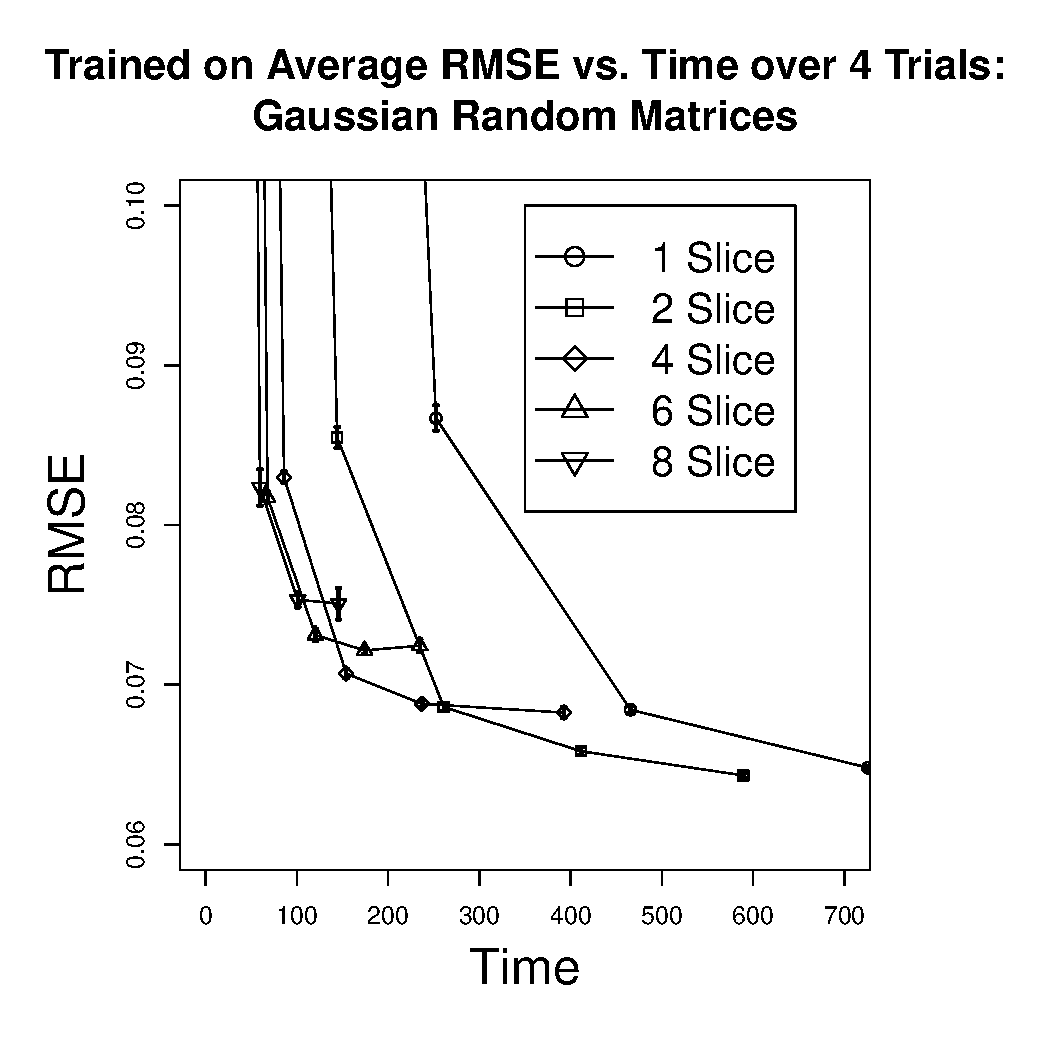
\includegraphics[width=\textwidth]{Graphs/4000_90_1_to_4_RvT_graph.pdf}}
		\caption{Training Data.}
\end{center}
	\end{subfigure}
\hspace{1cm}
	\begin{subfigure}[b]{.45\textwidth}
\begin{center}
		\fbox{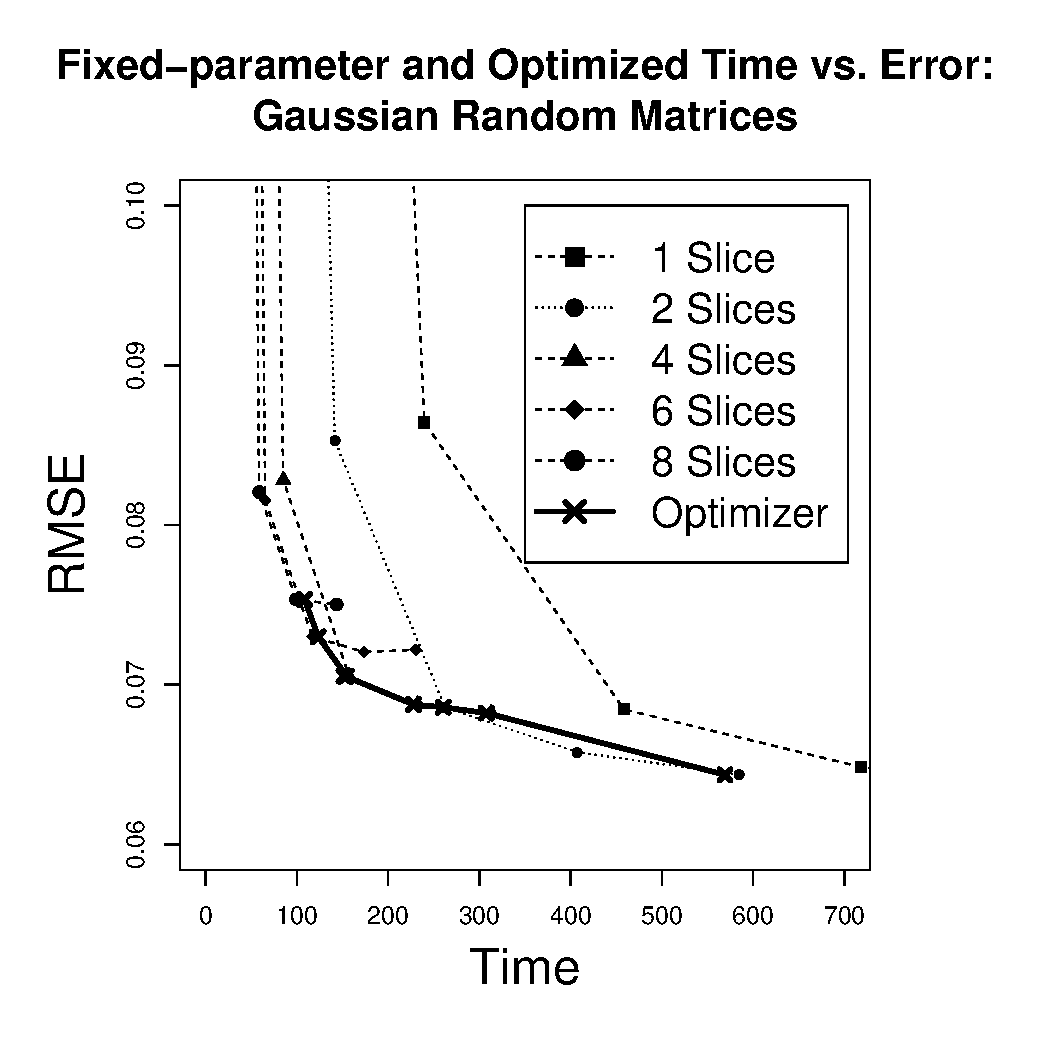
\includegraphics[width=\textwidth]{Graphs/Opt_Gaussian_4000.pdf}}
		\caption{Testing Data.}
\end{center}
	\end{subfigure}
\hfill
	\caption{Plots of Time and Error taken to factor a 4000 by 4000 matrix drawn from a Gaussian distribution.}	
\end{figure*}

\subsection{Movielens Data}
The second dataset we used to test the optimizer was the Movielens10M dataset. The Movielens dataset is a set of entries $(\text{UserID},\text{MovieID},\text{rating})$, with the rating parameter being a half-integer between $1$ and $5$. One can think of these three-tuples as specifying the entries of a matrix with rows and columns indexed by users and movies. 

The reason we might want to find a low-rank completion of this matrix is the assumption that there are a small number of properties that influence the way people rate movies. Then the two factors tell you how a person values each property, and how each movie is correlated with these properties. This lets you make predictions even on the hidden entries of the matrix, i.e. the movies a user has yet to see or rate. 

There are some qualitative differences between this data and the synthetic data in the previous section. The entries come from the range $[1,5]$ rather than being concentrated around zero, and thus the RMSE's for this section are much larger. The Gaussian matrices also come from a well-understood distribution so DFC comes with some theoretical guarantees and its behavior is pretty consistent across different random matrices. We have no such guarantee here, and we hope that the Movielens users behave similarly across partitions. 

The dataset was partitioned by the UserID into seven different pieces and the pieces were grouped to form the training/testing splits mentioned in the first section. Figure 2 displays the results of one of these splits. As before, each curve represents one of the choices of the division parameter in DFC. Once again we observe the intersection points where the division parameter should be changed for optimality to be satisfied. The bold line represents the optimized parameters for each budget. The graphs here are qualitatively the same as the graphs from the previous section. For every time budget, the optimizer picks the best division parameter. 

Table 2 summarizes the results of each of the training/testing splits for the Movielens dataset. Averaged over all these splits, the optimized parameter choices perform within [SOME NUMBER] of minimal error, and coming within [SOME NUMBER] of the budget.

\begin{figure*}
	\begin{subfigure}[b]{.45\textwidth}
\begin{center}
		\fbox{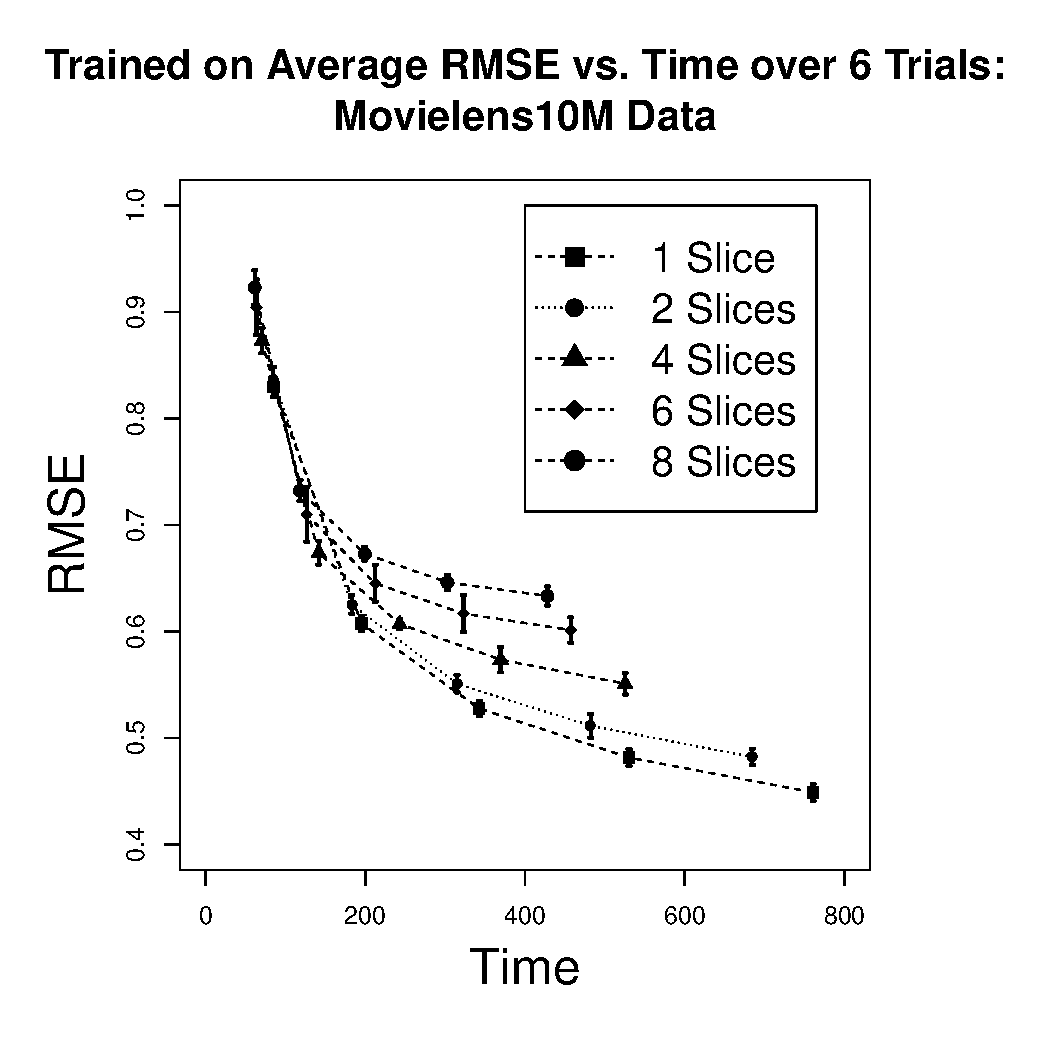
\includegraphics[width=\textwidth]{Graphs/movielens10M_1_to_4_RvT_graph.pdf}}
		\caption{Training Data.}
\end{center}
	\end{subfigure}
\hspace{1cm}
	\begin{subfigure}[b]{.45\textwidth}
\begin{center}
		\fbox{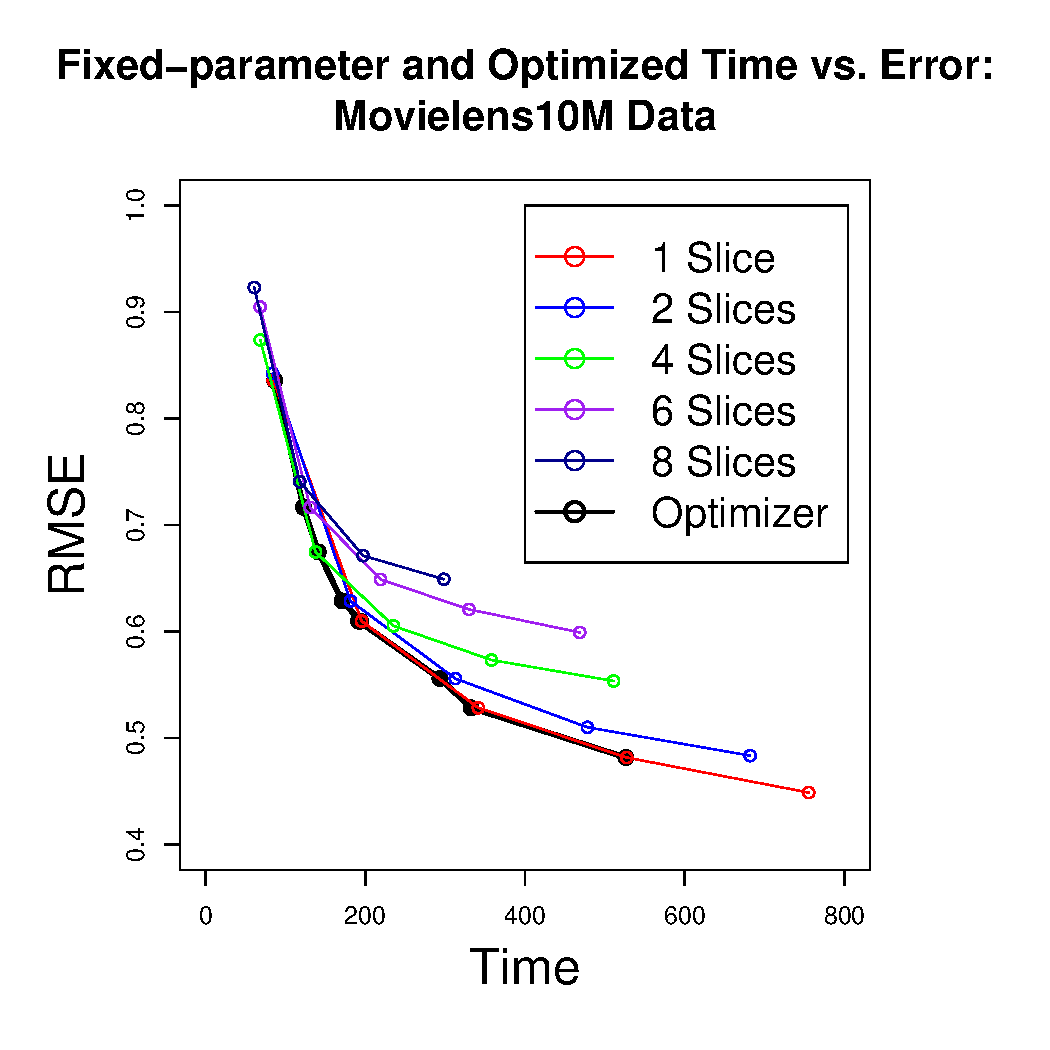
\includegraphics[width=\textwidth]{Graphs/Opt_movielens.pdf}}
		\caption{Testing Data. }
\end{center}
	\end{subfigure}
\hfill
	\caption{Plots of Time and Error taken to factor the Movielens10M Dataset partitions.}	
\end{figure*}

\subsection{Testing Explore Mode}
The previous sections show that our optimizer performs quite well when its training set accurately reflects the behavior of the algorithm on future jobs. However, sometimes an application can receive an instance that is unlike the previously seen jobs. In this case, we want to use some randomness while picking our parameters so that we can explore the parameter space. We would like to explore without sacrificing too much in the error or time of the computation, so we pick parameters proportionally to the error we expect to get with those settings. 

We tested this functionality by beginning with estimations for small Gaussian inputs and feeding the optimizer larger matrices. We gave the optimizer training data from $2000 \times 2000$ Gaussian random matrices and applied our estimation method to guess runtime profiles for $4000 \times 4000$ Gaussian random matrices. Finally, we gave the optimizer a sequence of ten $4000 \times 4000$ Gaussian random matrices and asked the computation to finish within two-hundred seconds. While exploring, the optimizer was able to find a parameter setting with an error that was within $15\%$ of the best parameter choice that satisfies that budget that we could find in hindsight. It did not find better settings because we over-estimated the amount of time per iteration, and so the optimizer did not try running with more iterations because it thought that would violate the budget.